\chapter{Summary and Conclusion}
\label{results}
\qquad This chapter summarizes the main results of the undertaken MSc by Research 2018 project and describes its workflow as it happened. In short, the main results of the undertaken MSc by Research project can be described with several points:
\begin{enumerate}[align=left,leftmargin=*]
\item \textbf{Software source code parallelizability metrics search has been conducted. MSc by Research project has been set up.}\newline
\null\qquad A body of literature has been searched through in an attempt to find any software source code metrics, applicable to the software parallelizability problem. While there are a lot of metrics aimed at judging about software quality (maintainability, readability, etc.), none were proposed to judge about software parallelizability. The only metrics in the subfield of parallel computation represent different variations of program execution time speedup ratio. Short report is given in the sections \ref{background-software-metrics-in-cs} and \ref{background-metrics-parallel-computing} of the background chapter \ref{backgroud}.\newline
\null\qquad It was decided, that Program Dependence Graph (PDG) (proposed in the paper \cite{pdg-paper}) is going to be an intermediate program representation, parallelizability metrics would be computed on. Moreover, parallelizability metrics would use loop decoupling and loop iterator recognition results (proposed in the paper \cite{iterator-recognition-paper}) as a prerequisite for their further computation. The first metric to be computed was decided to be \textit{loop payload fraction} (see \ref{metrics-loop-payload-fraction}). LLVM compiler components library \cite{llvm-official-website},\cite{llvm-paper} was chosen for the MSc project to be based on.	
\item \textbf{Development of LLVM-based metric computing tool.}\newline 
\null\qquad This stage took the most of the time and efforts. As a result PPar tool (described in \ref{ppar-tool} and hosted on the GitHub \cite{ppar-tool}) ($\approx$ 4750 C/C++ lines of code) has been developed. The tool development started straight after the first metric ideas were conceived (end of January 2018).\newline
\null\qquad The PDG intermediate representation and all algorithms, proposed and described in \cite{pdg-paper} and \cite{iterator-recognition-paper} have been implemented from the scratch. This took a significant project start-up overheads. Development of dependence graph intermediate representation on top of LLVM IR along with loop decoupling and iterator recognition algorithms (strongly connected components search) alone took more than a month of time. During that period LLVM's DEBUG() prints served as the only debugging and validation means.\newline
\null\qquad After the first graph visualization facilities (see section \ref{ppar-tool-graph-visualizations}) (thanks to Graphviz and DOT) had been added the project, the first research work has actually started. Along with further validation, debugging and development of the tool, first metrics started to appear on the small hand-written tests. Metric values have been manually validated against PDG and its SCCs DOT graph visualizations. Visualizations of these PDG and their SCCs served as an inspiration for the proposal of a new metrics.\newline
\null\qquad By June 2018, 17 metrics have been devised and integrated into the developed PPar tool framework. Metric values could be obtained on the small set of hand-written tests. These values have been manually verified with graph visualizations. This work has been reported during the Intermediate Progress Review held on the 7$^{th}$ of June 2018.                    
\item \textbf{Devised metric values have been collected on the NAS benchmark suite.}\newline
\null\qquad In the beginning of June PPar tool got to a relatively stable state, and work moved from small hand-written tests onto SNU NAS benchmarks implementations. Thanks to another PhD student Chris Vasiladiotis, who kindly provided his CMake-based testing infrastructure, running of these NAS benchmarks through the PPar tool started almost immediately and I managed to jump over technical difficulties straight to getting first research results.      
	
\item \textbf{Analysis of devised parallelizability metrics.}\newline
\null\qquad Once all metric values had been gathered for all NAS benchmark loops and all loops had been classified with Intel C/C++ compiler, the final analytic stage of the project could be started. All analysis results are available in the chapter \ref{analysis} of the thesis.\newline
\null\qquad Devised and proposed software metrics for parallelism have been examined and looked at from different angles and with different techniques:
\begin{enumerate}
\item \textbf{Single metric analysis and visualizations.}\newline
\null\qquad Collected metric values had been visualised with the help of Python, pandas \cite{python-lib-pandas} and matplotlib \cite{python-matplotlib}, and these plots had been visually examined on the subject of parallelizability correlations. These examinations showed that correlations are weak and take place only for certain metrics. The strongest correlations were observed for \textit{iterator/payload total} and \textit{non-CF cohesion} metrics, \textit{critical payload fraction} and \textit{payload fraction metrics}. But still correlations have probabilistic and statistical nature.\newline 
\null\qquad For example, if $\textit{iterator/payload non-cf cohesion} \ge 0.029$, then the loop is going to be parallelizible/non-parallelizible with probabilities 59\% and 41\% correspondingly. If, on the other hand, $\textit{iterator/payload non-cf cohesion} \le 0.029$, then the loop is going to be non-parallelizible with probability of 75\%. Such answers are not much better (if at all) than Intel compiler's binary "yes"/"no" answers. All these results can be looked at section \ref{analysis-data-interpretation-and-visualization}.\newline  

\item \textbf{Principal Component Analysis (PCA) and clustering of combined metric set.}\newline
\begin{figure}[H]
\centering
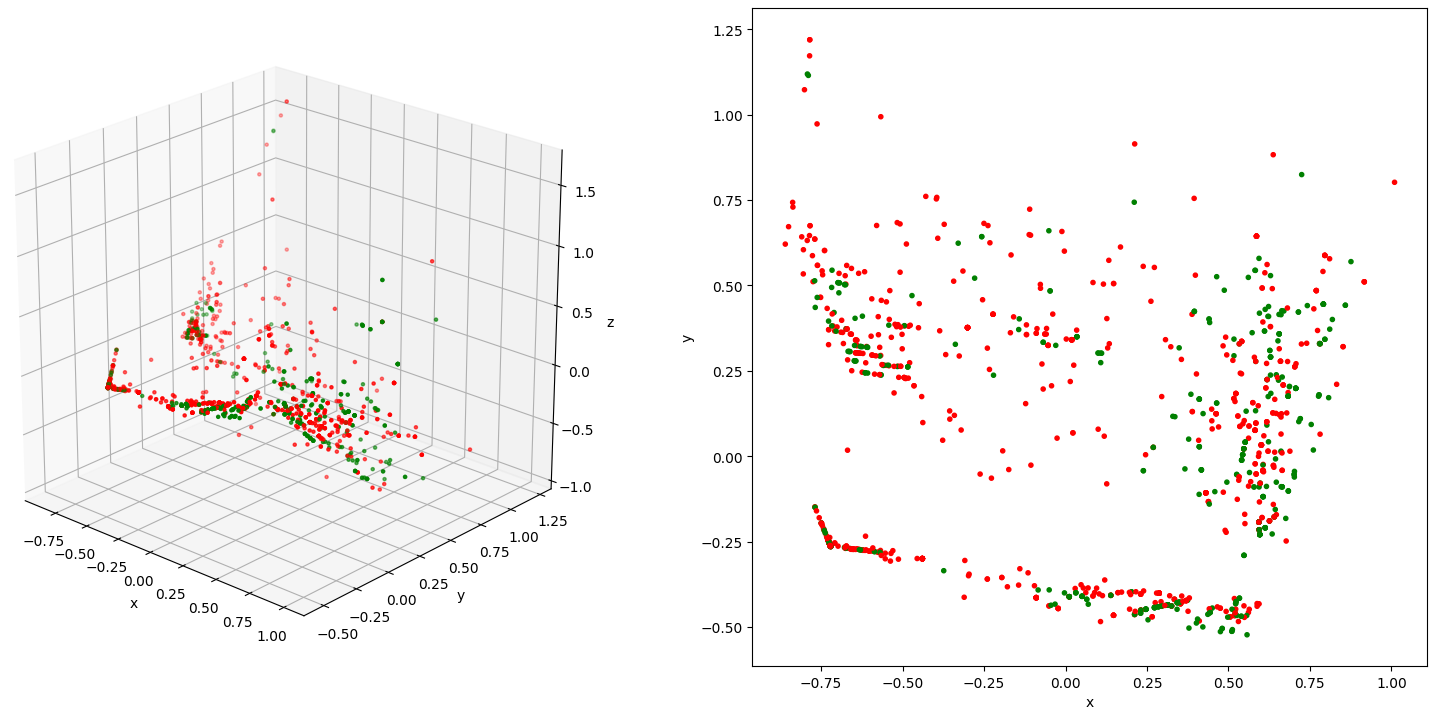
\includegraphics[width=\linewidth]{figs/metrics-pca-parallelizability.png}
\caption{}
\label{results-clustering}
\end{figure}
\null\qquad All metrics have been considered altogether with the help of Principal Components Analysis (PCA) and clustering techniques. Figure \ref{results-clustering} shows the results of PCA application to the whole set of metrics.\newline
\null\qquad Despite the fact, that metrics dataset 3D projection shows some some structural patterns (condensed clots of loops) (see section \ref{analysis-data-clustering-analysis}), parallelizability property distributed all across the whole space, intermixing parallelizible (green) loops (dots) with non-parallelizible (red) loops (dots).\newline 

\item \textbf{Decision tree based visualisation.}\newline
\null\qquad Figure \ref{results-decision-tree} shows the decision tree, built by scikit-learn \cite{python-lib-scikit-learn} Python machine learning (ML) library. Decision tree uses mathematical foundations to study dataset and generate the tree of classification (parallelizible or not) derivation.\newline 
\null\qquad Decision tree algorithm picked up the best metrics for the task of parallelizability classification and put them closer to the root of the tree. As it can be seen, these metrics correspond to the ones, found to be the most correlating during single metric visualizations (see \ref{analysis-data-interpretation-and-visualization} and (a)).\newline
\null\qquad If we use several metrics to classify loops, according to the decision tree \ref{results-decision-tree}, then we might get better probabilities. For example if we use the following system of metric inequalities to filter loops we are going to get roughly 65\% probability of a loop being parallelizible. 
\begin{equation*}
\begin{cases}
\begin{aligned}
\textit{iterator-payload non-cf cohesion}            &\ge 0,029 \\[1ex]
\textit{iterator-payload total cohesion} &\ge 0.21 \\[1ex]
\textit{loop-critical-payload-fraction} &\leq 0.349
\end{aligned}
\end{cases}
\end{equation*}\newline
\begin{sidewaysfigure}
\centering
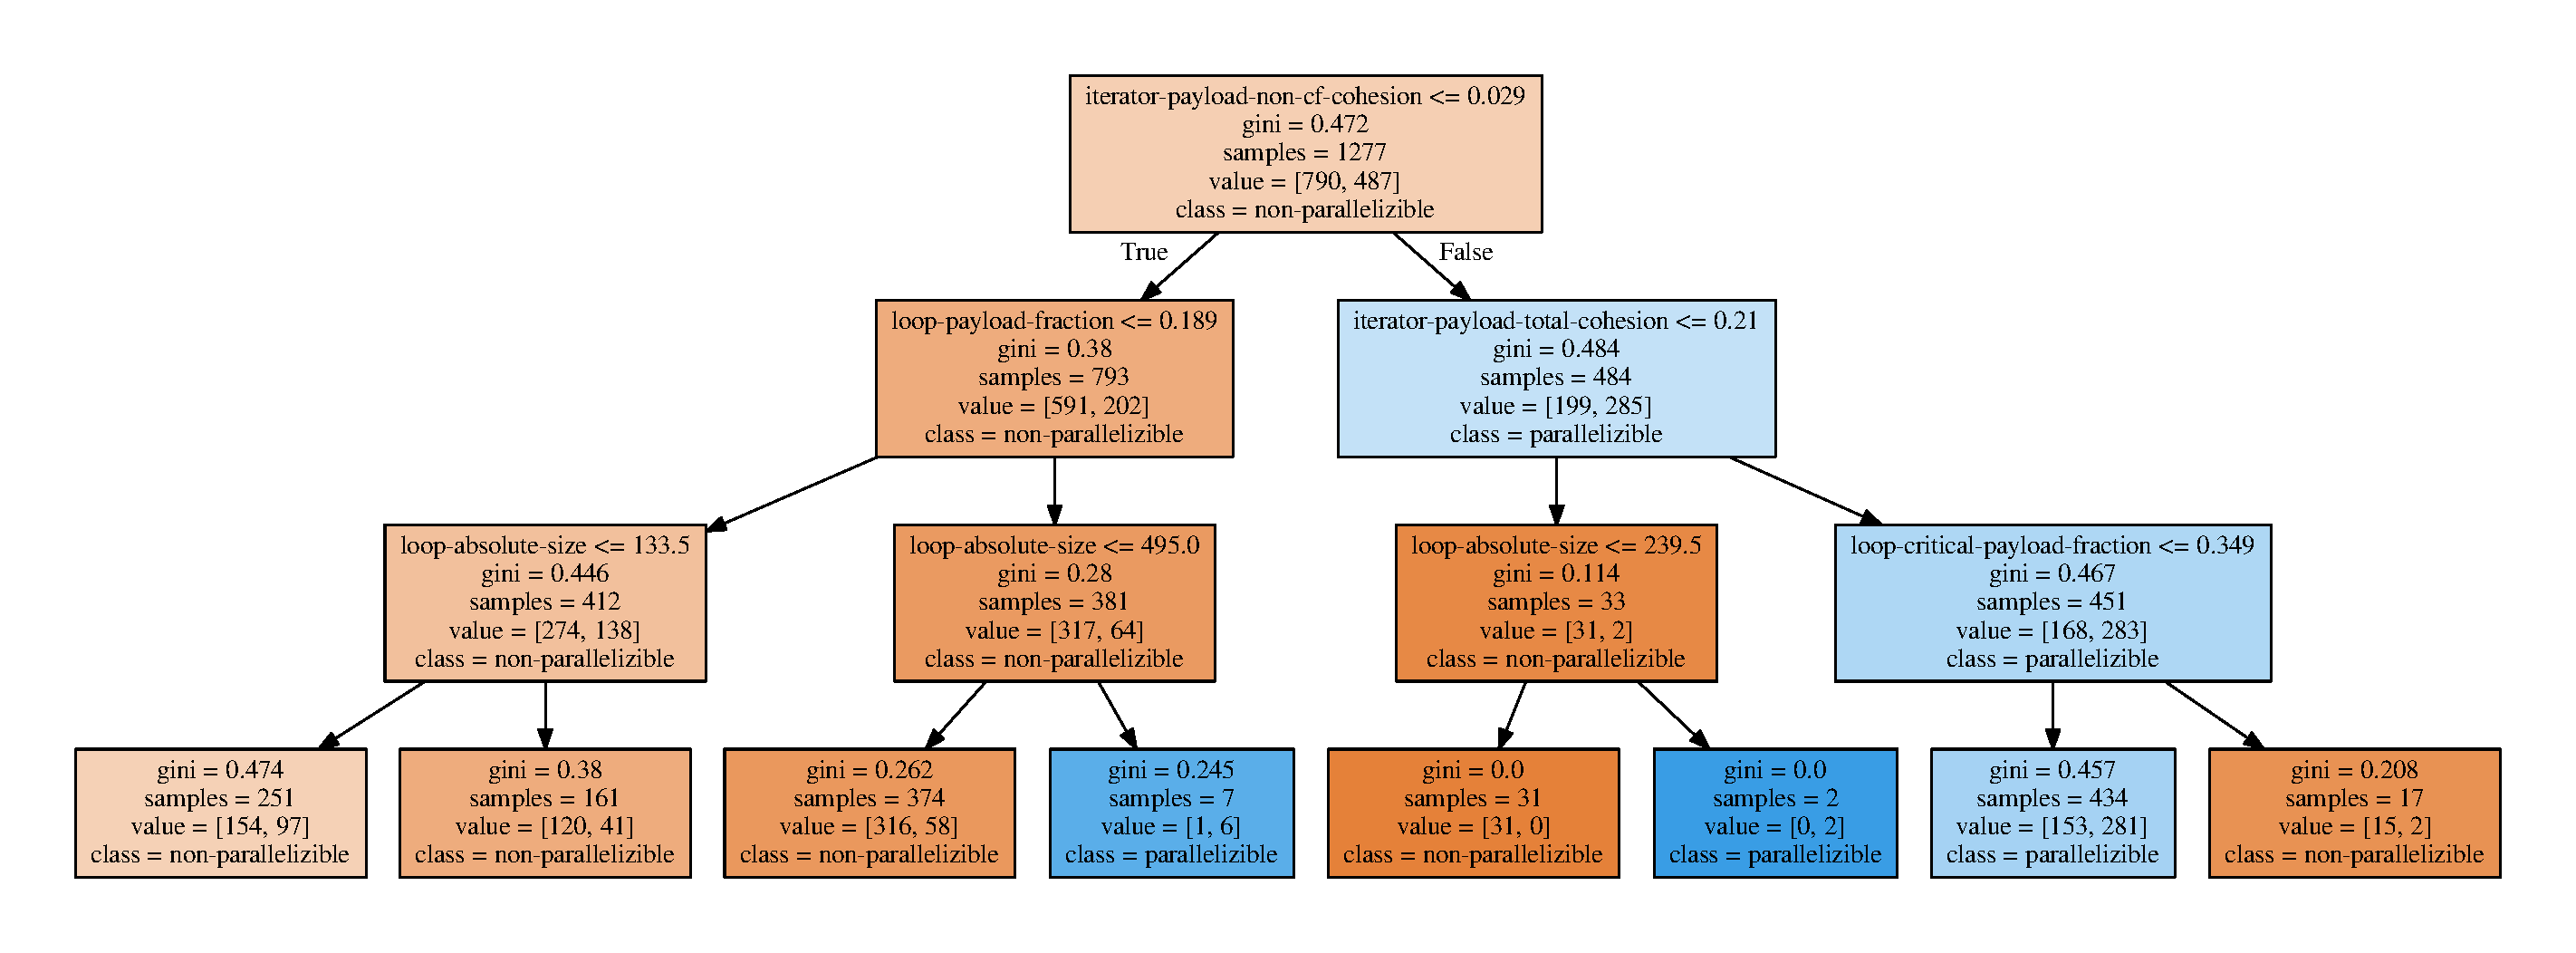
\includegraphics[width=\linewidth]{figs/decision-tree-depth-3.pdf}
\caption{Dataset \ref{analysis-data-table} decision tree, limited to the depth of 3.}
\label{results-decision-tree}
\end{sidewaysfigure}

\item \textbf{Manual analysis of benchmarks source code, Intel compiler reports and software parallelizability metrics.}\newline
\null\qquad Section \ref{analysis-manual-analysis} presents some source code listings, where Intel ICC compiler faile to parallelize some algorithmically parallelizible loops, but metric-based decision tree classifier gives them correct classification. Such loops mostly have to do with inaccuracies of compiler's alias and dependence analysis. 

\item \textbf{Machine learning techniques.}\newline 
\null\qquad And finally, different statistical learning techniques have been applied to the dataset of metric values, in order to estimate prediction accuracies of trained models. If random classifications are going to get us approximately 50\% accuracy, then if we use the whole set of 13 metrics as ML features we are going to get about 77\% prediction accuracy with decision tree methods. This shows, that proposed metrics manage to capture some parallelizability properties of software loops and work the best altogether. More detailed report can be found in the section \ref{analysis-statistical-analysis} of the thesis.
\end{enumerate}

\end{enumerate}
\qquad The overall picture in the matter of software source code (loops in particular) metrics for  parallelisability resembeles that of the software quality metrics. Software quality (say, maintenance) is a complex notion. To judge about "good" or "bad" software design one must posses vast software engeeniring expertise and skills. Metrics like cyclomatic complexity can be used as supplementary to manual analysis, but the values they give must be examined by a human with a deep understanding of the software quality question. Although, their values might sometimes correlate with the understanding of a sound software design, these metrics should not be applied blindly.\newline
\null\qquad Software parallellizability property is not a simplier one. Despite the fact, that all examined metrics have grounds to be proposed and are not randomly selected, their parallelizability correlations are limited and there are always special cases, which break generally established rules and patterns.\newline
\null\qquad However, the working framework, developed withing that MSc by Research project, is ready and can be used for further metrics research and analysis. It is quite easy to add new metrics to the tool. Tool provides visualization facilities for dependence graphs and loop iterator/payload decomposition. New metrics might be added. Alternatively, existing metrics might be fine-tuned as well.\newline 
\null\qquad This work might be the one on the relatively new direction - application of machine learning in compilers. Since all machine learning methods require some quantitative features, these loop metrics might be an attempt in their establishment. Modern compilers apply a set of optimizations: loop unrolling, peeling, splitting. Correlations between these metrics and these properties (like loop unrollability) might be examined towards development of machine-learning driven compiler optimizers.      